\documentclass[a4paper,10pt]{article}
\usepackage[margin=2.5cm]{geometry}
\usepackage[utf8]{inputenc}
\usepackage[colorlinks=true,urlcolor=blue]{hyperref}
\usepackage{amsmath}
\usepackage{graphicx}
\usepackage{float}
\usepackage{caption}
\usepackage{subcaption}
\usepackage{xcolor}
\usepackage{booktabs}

\usepackage{listings} %Alternative to minted
\definecolor{codegreen}{rgb}{0,0.6,0}
\definecolor{codegray}{rgb}{0.5,0.5,0.5}
\definecolor{codepurple}{rgb}{0.58,0,0.82}
\definecolor{backcolour}{rgb}{0.95,0.95,0.92}
 
\lstdefinestyle{mystyle}{
    backgroundcolor=\color{backcolour},   
    commentstyle=\color{codegreen},
    keywordstyle=\color{magenta},
    numberstyle=\tiny\color{codegray},
    stringstyle=\color{codepurple},
    basicstyle=\footnotesize,
    breakatwhitespace=false,         
    breaklines=true,                 
    captionpos=b,                    
    keepspaces=true,                 
    numbers=left,                    
    numbersep=5pt,                  
    showspaces=false,                
    showstringspaces=false,
    showtabs=false,                  
    tabsize=2
}

\lstset{style=mystyle}
\setlength{\parindent}{0em}
\setlength{\parskip}{1em}
% figure support
\usepackage{import}
\usepackage{xifthen}
\pdfminorversion=7
\usepackage{pdfpages}
\usepackage{transparent}

\pdfsuppresswarningpagegroup=1

\title{Learning to play Pong with DQN}
\author{Group 21 - Linus Falk}
\begin{document}
\maketitle
\section{Introduction}
This project is part of the Reinforcement learning 7.5c course at Uppsala University. We are asked to implement the Deep Q-network that was first introduced by Mnih et.al \cite{dqn1}. In order to simplify the work and debugging of the code we were first asked to implement it in a simple environment such as the CartPole and after that move on to the more challenging Pong environment \cite{gym}.  

\section{Deep Q-network (DQN)}
Deep Q-network is a Reinforcement learning algorithm that combines the use of neural networks and the classic reinforcement learning technique, Q-learning. In Q-learning the agent learns the Q(s,a) function which estimates the total reward that can be obtained by taking an action \emph{a} in state \emph{s}, where \emph{a} $\in \mathcal{A}$ and \emph{s} $\in \mathcal{S}$, the action and state spaces. This function can be solved by using the Bellman equation when the state and action spaces are small \cite{sutton}. However, in most application that is not the case and we most use function approximation instead of a matrix of action and states. Using deep learning methods is one way to solve it could be hard to train since the most deep learning algorithms expects that the data samples to be independent of each other, this is not often the case in Reinforcement learning. To overcome the obstacles of using deep learning methods to model more complex action spaces was these solutions proposed \cite{dqn1}.        


\begin{itemize}
	\item \textbf{Experience Replay}
	\item \textbf{Target network}
\end{itemize}

In order to solve the correlation problem was the \textbf{Experience replay} introduce that stores sequences of state, action, reward and next state. When training the replay buffer is sampled to update the network which helps to break the correlation between consecutive samples\cite{dqn1}. The \textbf{Target network} was introduced to stabilize the training that was often unstable when generating the target with the same model that could affect the action values for the next step leading to catastrophic forgetting of learning. By using a model that is not updated immediately and uses old parameters it was possible to get more stable training \cite{dqn2}    

\section{Cartpole-v1}
The Cartpole model was implemented using the Gymnasium tool kit for Reinforcement learning and with skeleton code provided by the instructor. The neural network was in this case very simple, see table: \ref{tab:polearc}:
\newpage

\begin{table}[h]
\centering
\begin{tabular}{|c|c|c|}
\hline
\textbf{Layer (type)} & \textbf{Input Shape} & \textbf{Output Shape} \\
\hline
Linear 1 & 4 & 256 \\
\hline
ReLU &  &  \\
\hline
Linear 2 & 256 & 2 \\
\hline
\end{tabular}
\caption{Neural Network Architecture}
\label{tab:polearc}
\end{table}

The model was then trained with different hyperparameters to see how it affected the training and result. The hyperparameters common for all model are presented i table: \ref{tab:cartpole1} and the hyperparameters that was change are presented in table: \ref{tab:cartpole2}. To evaluate the training was the training stopped and evaluated periodically and tested for 5 times and the mean return was then plotted over the course of the training. The average return of these evaluations during training are presented in figures: \ref{fig:image1} to \ref{fig:image5}. 



\begin{table}[ht]
\centering
\begin{tabular}{|l|l|}
\hline
\textbf{Hyperparameter} & \\
\hline
memory\_size & 50000 \\
n\_episodes & 1000 \\
batch\_size & 32  \\
lr & 1e-4 \\
train\_frequency & 1\\
gamma & 0.95  \\
anneal\_length & 10$^4$ \\
n\_actions & 2 \\
\hline
\end{tabular}
\caption{Hyperparameters for CartPole-v1}
\label{tab:cartpole1}
\end{table}


\begin{table}[ht]
\centering
\begin{tabular}{|l|l|l|l|l|l|}
\hline
\textbf{Hyperparameter} & \textbf{Model 1} & \textbf{Model 2} & \textbf{Model 3} & \textbf{Model 4} & \textbf{Model 5} \\
\hline
target\_update\_frequency & 100 & 5 & 150 & 100 & 100 \\
gamma & 0.95 & 0.95 & 0.95 & 0.95 & 0.95 \\

eps\_start & 1.0 & 1.0 & 1.0 & 0.5 & 1.0 \\
eps\_end & 0.05 & 0.05 & 0.05 & 0.05 & 0.5 \\
\hline
\end{tabular}
\caption{Hyperparameters for CartPole-v1}
\label{tab:cartpole2}
\end{table}



\begin{figure}[htbp]
  \centering
  \begin{subfigure}{0.3\textwidth}
    \includegraphics[width=\textwidth]{figures/CartPole_history_1.png}
    \caption{Model 1}
    \label{fig:image1}
  \end{subfigure}
  \hfill
  \begin{subfigure}{0.3\textwidth}
    \includegraphics[width=\textwidth]{figures/CartPole_history_2.png}
    \caption{Model 2}
    \label{fig:image2}
  \end{subfigure}
  \hfill
  \begin{subfigure}{0.3\textwidth}
    \includegraphics[width=\textwidth]{figures/CartPole_history_3.png}
    \caption{Model 3}
    \label{fig:image3}
  \end{subfigure}
  \label{fig:all_images}

  \vfill


  \begin{subfigure}{0.3\textwidth}
    \includegraphics[width=\textwidth]{figures/CartPole_history_4.png}
    \caption{Model 4}
    \label{fig:image4}
  \end{subfigure}
  \label{fig:both_images}
   \hfill
  \begin{subfigure}{0.3\textwidth}
    \includegraphics[width=\textwidth]{figures/CartPole_history_5.png}
    \caption{Model 5}
    \label{fig:image5}
  \end{subfigure}
  \label{fig:both_images}
\end{figure}



\subsection*{Discussion}
Looking at the return plots of the different models we can see that reducing the \emph{target update frequency} (in model 2) lead to a better model with higher return. The correlation problem was perhaps not that big in this simple environment, but we can see some tendency that it fluctuates more than the previous model. Dialing the \emph{target update frequency} up showed instead that the training became too slow/stable and didn't learn enough the environment to improve. In model 4 and 5 the exploration strategy's was changed by changing the probability for exploration during the training. Model 4 with less experience in the beginning show slower progress than model 1 which is expected. Model 5 on the other hand keeps a high degree of exploration and is instead not able to find a more optimal policy do to this, giving it a smaller overall return than model 1 and 2.  

The implementation of this environment was straight forward with the skeleton given and easy to understand \#TODO's. Some problems and perhaps a deviation from strategy thought of the instructor was done with the masking of the terminating states. Here was an integer introduce to "mask" the terminated samples. A simple mistake of not updating state to the next state in the end of the training loop gave more headache than i should. 

\newpage 
\begin{lstlisting}
obs = torch.tensor(obs).to(device)
next_obs = torch.tensor(next_obs).to(device)
action = torch.tensor(action).unsqueeze(0).to(device)
reward = torch.tensor(reward).unsqueeze(0).to(device)

if terminated:
  terminated_bool = torch.tensor(1).unsqueeze(0)
else:
  terminated_bool = torch.tensor(0).unsqueeze(0)

memory.push(obs, action, next_obs, reward, terminated_bool)

###########

Q_targets = concatenated_reward + (dqn.gamma * max_next_q_values * (1 - concatenated_terminated))
\end{lstlisting}





\section{Atari - Pong}
The next step was to train a model for the Atari-Pong environment. The code from the previous environment could mostly be reused but new hyperparameters that would "guarantee" a reasonably good training was given, see table: \ref{tab:hyperparameters}. The Neural network was also updated to a Convolutional Neural Network, CNN. The architecture is presented in figure: \ref{fig:arcpong}.  

\begin{table}[ht]
\centering
\begin{tabular}{|c|c|}
\hline
\textbf{Hyperparameter} & \textbf{Value} \\
\hline
Observation stack size & 4 \\
Replay memory capacity & 10000 \\
Batch size & 32 \\
Target update frequency & 1000 \\
Training frequency & 4 \\
Discount factor & 0.99 \\
Learning rate & 1e-4 \\
Initial epsilon & 1.0 \\
Final epsilon & 0.01 \\
Anneal length & 10$^6$ \\
\hline
\end{tabular}
\caption{Hyperparameters}
\label{tab:hyperparameters}
\end{table}

\begin{figure}[ht!]
\centering
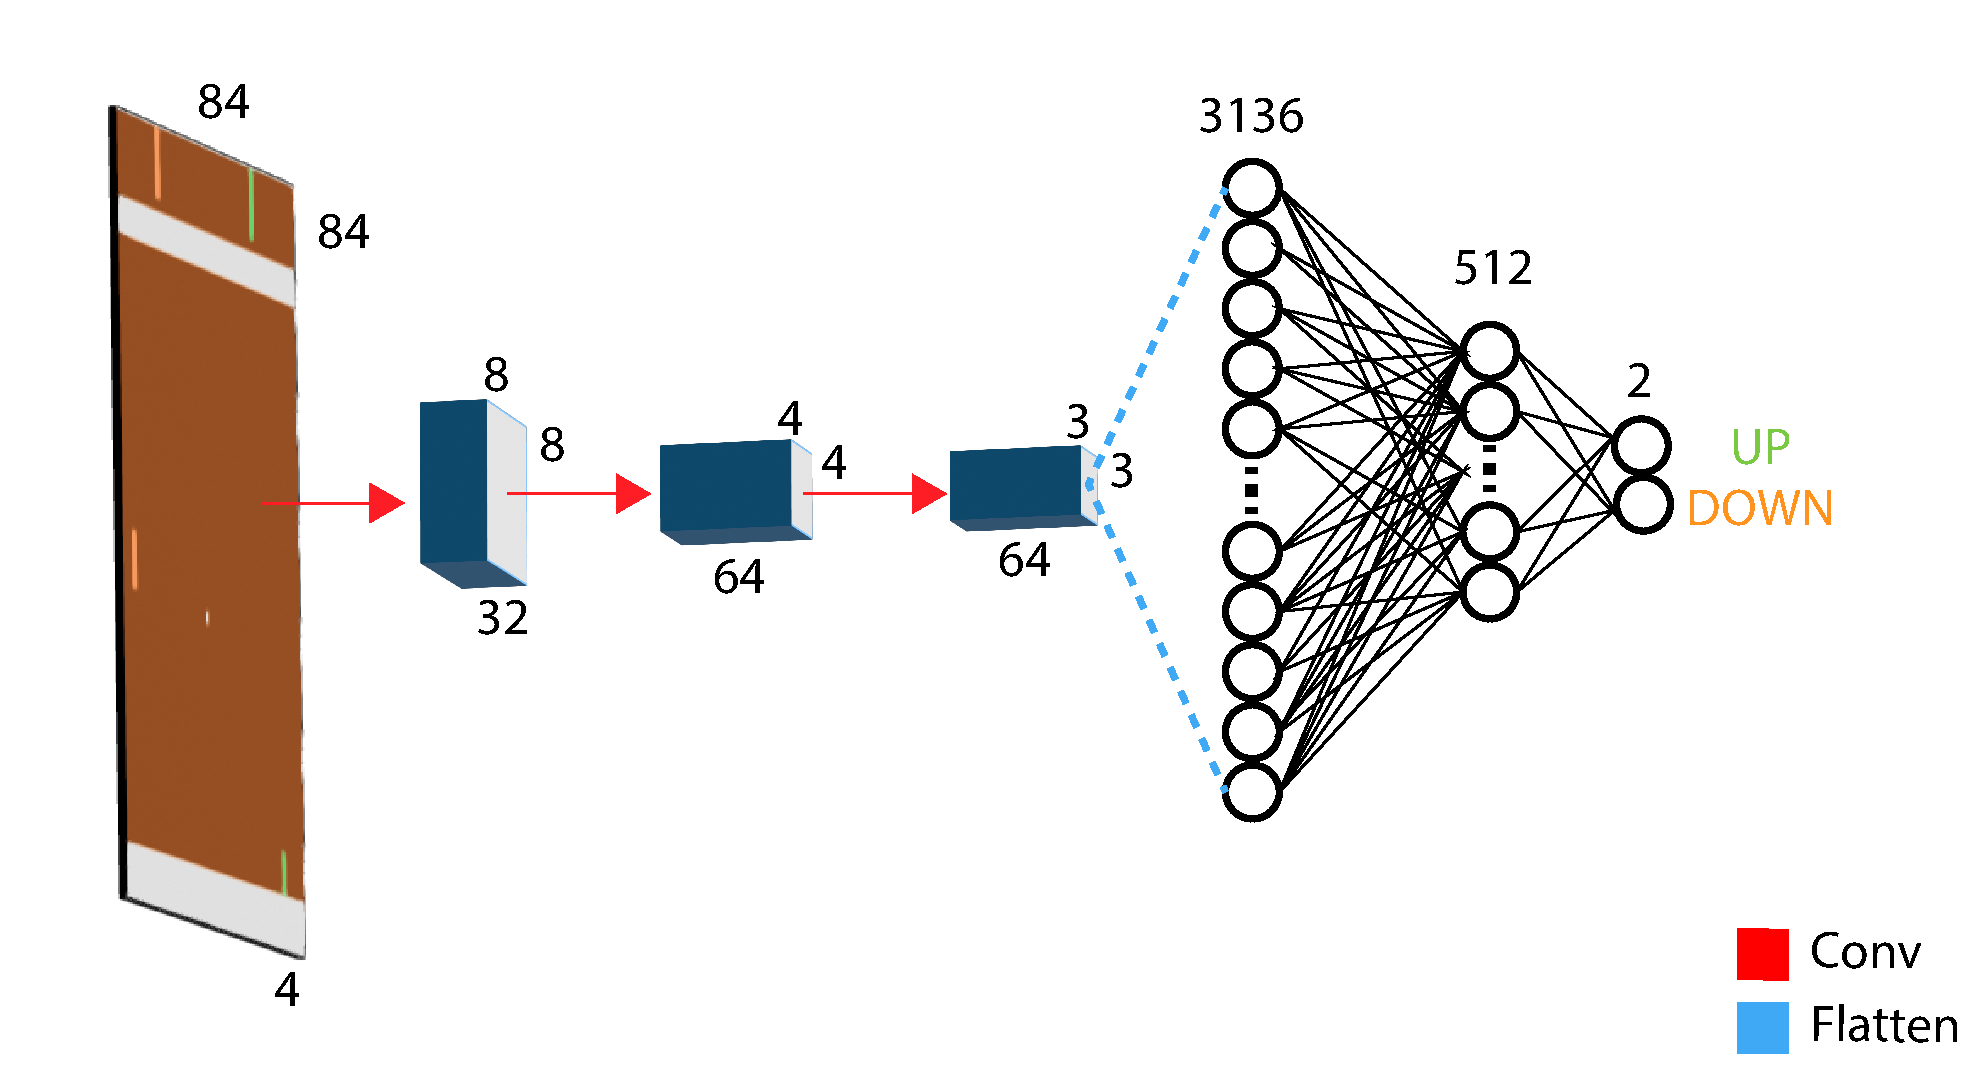
\includegraphics[width=130mm]{figures/DQN.pdf}
\caption{CNN architecture}
\label{fig:arcpong}
\end{figure}


\begin{figure}[ht!]
\centering
\includegraphics[width=0.5\textwidth]{figures/Pong_history_1.png}
\caption{Neural network architecture}
\label{fig:pongresult}
\end{figure}


\newpage 

\subsection*{Discussion}
The most challenging part of this part was to get the stacking of the sequence of images that was collected from the environment and save them to the replay memory correctly. But the instructions given in the task helped and the problem was solved eventually. After overcoming these minor obstacles the work was not that difficult until it was time to start to test. One of the challenges was to see if it was correctly implemented and actually could improve its policy. The training took typically around 5-6 hour training it on a \emph{Nvidia RTX3060}, with not much improvement the first 5-10 minutes. The result is present in figure: \ref{fig:pongresult}. The episode on the x-axis is the number of the evaluation episode that was done every 25th normal episode.   



\begin{thebibliography}{1}

\bibitem{dqn1} Volodymyr Mnih and Koray Kavukcuoglu and David Silver and Alex Graves and Ioannis Antonoglou and Daan Wierstra and Martin Riedmiller (2013). Playing Atari with Deep Reinforcement Learning

\bibitem{gym} Brockman, Greg and Cheung, Vicki and Pettersson, Ludwig and Schneider, Jonas and Schulman, John and Tang, Jie and Zaremba, Wojciech (2016). Openai gym

\bibitem{sutton} Richard S. Sutton and Andrew G. Barto (2018). Reinforcement learning - An introduction

\bibitem{dqn2} Mnih, V., Kavukcuoglu, K., Silver, D. et al (2015) Human-level control through deep reinforcement learning.

\end{thebibliography}

\end{document}